%%%%%%%%%%%%%%%%%%%%%%%%%%%%%%%%%%%%%%%%%%%%%%%%%%%%%%%%%%%%%%%%%%%%%%%%%%%%%%%%
%2345678901234567890123456789012345678901234567890123456789012345678901234567890
%        1         2         3         4         5         6         7         8

%\documentclass[letterpaper, 10 pt, conference]{ieeeconf}  % Comment this line out if you need a4paper

\documentclass[a4paper, 10pt, conference]{ieeeconf}      % Use this line for a4 paper

%\IEEEoverridecommandlockouts                              % This command is only needed if 
                                                          % you want to use the \thanks command

\overrideIEEEmargins                                      % Needed to meet printer requirements.

% See the \addtolength command later in the file to balance the column lengths
% on the last page of the document

% The following packages can be found on http:\\www.ctan.org
\usepackage{graphicx} % for pdf, bitmapped graphics files
\usepackage{subcaption}
%\usepackage{epsfig} % for postscript graphics files
%\usepackage{mathptmx} % assumes new font selection scheme installed
%\usepackage{times} % assumes new font selection scheme installed
%\usepackage{amsmath} % assumes amsmath package installed
%\usepackage{amssymb}  % assumes amsmath package installed
\graphicspath{{figure/}}
\title{\LARGE \bf
Practical robotic course: Project Grasp
}


\author{Nguyen Truong Thinh$^{1}$ and Mengnan Wang$^{2}$% <-this % stops a space
\thanks{*This work was not supported by any organization}% <-this % stops a space
}


\begin{document}


\maketitle
\thispagestyle{empty}
\pagestyle{empty}


%%%%%%%%%%%%%%%%%%%%%%%%%%%%%%%%%%%%%%%%%%%%%%%%%%%%%%%%%%%%%%%%%%%%%%%%%%%%%%%%
\begin{abstract}
In this project, we develop a system to solve grasping single object in 2D plane. We apply reinforcement learning on moving robot arm to object in 2D plane based on vision and supervised learning on choosing grasping point. Grasping points are learnt from synthetic images and then used on novel objects. The result shows that our system can grasp single object which is similar to training examples.   

\end{abstract}


%%%%%%%%%%%%%%%%%%%%%%%%%%%%%%%%%%%%%%%%%%%%%%%%%%%%%%%%%%%%%%%%%%%%%%%%%%%%%%%%
\section{INTRODUCTION}
Robotic grasping novel object is still an unsolved problem in robotic community. Although it is an easy task for human, developing robotic systems that can mimic human grasping behavior is difficult.

In our project, we try to solve the grasping task in 2D plane instead of 3D space. The object always lies in a 2D plane and grasping is performed from above.
\section{BACKGROUND}
Recent researches focus on using deep neuron network to solve grasping task. They map the vision of robot to a joint configuration of robot arm. Such method often requires much training time, since training is applied on real robot instead of simulation\cite{c1}. The tuning of neuron network is also state-of-art.

Another method to solve robot grasping is dividing grasping task into multiple small tasks. This involves prior knowledge from human, which simplifies the whole task. Although this method sounds like hard-coded and less research-oriented, it is efficient in solving grasping task and learning framework can be applied on subtasks to make it 'intelligent'.

Usually, the grasping task is divided into choosing grasping point, estimating grasping configuration and executing grasping. First, grasping point is chosen based on the information of object image. Then a 3D position and orientation is estimated. Finally the gripper will execute the estimated 3D position and orientation.

\section{SYSTEM DESCRIPTION}
 We divide grasping task into four sub-tasks instead of three, approaching object in 2D plane, choosing grasping point, estimating 3D position and orientation and executing grasping.
\subsection{Approach object in 2D plane}
\begin{figure}
	\centering
	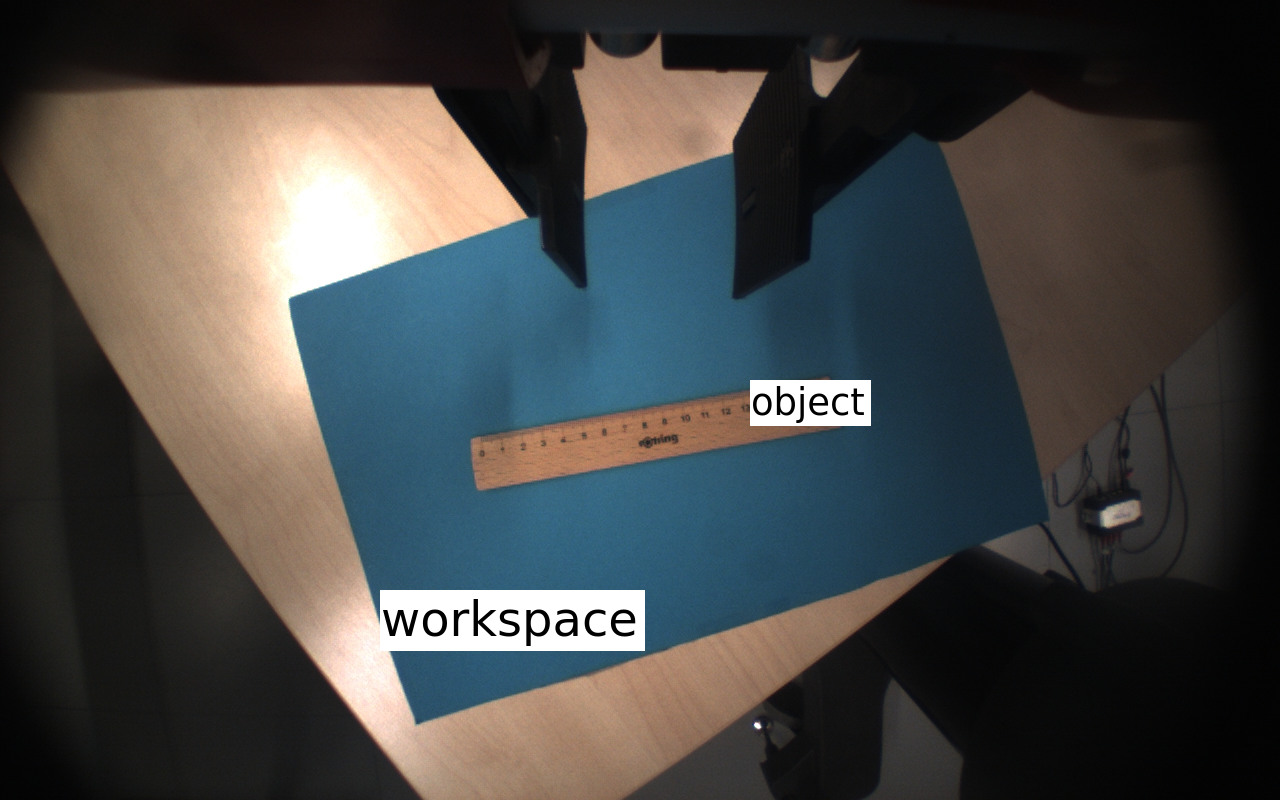
\includegraphics[width=0.8\linewidth]{workspace}
	\caption{\label{fig:workspace}Workspace}
\end{figure}
Before moving the arm to object, we first extract the object contour from image. We have a blue board as workspace, shown in figure \ref{fig:workspace}. First we use color filter to detect the convex hull of workspace. Then we use background subtraction to extract contour of object inside our workspace. We further compute the centroid of object. 

To approach object in 2D plane, we use reinforcement learning. The problem is formulated as a Markov Decision Process. Given the vector points from centroid of object to the image center, the arm has four actions forward/backward/left/right and the step size of each action is about 1cm. The goal state is reached when the center of camera is roughly align with the centroid of object. 

We try two learning frameworks. The tabular Q-learning\cite{c2} and Least Square Policy Iteration(LSPI)\cite{c3}. The vector points from centroid of object to center of camera describes the relative position of object to gripper center. 
\begin{figure}[!htb]
	\centering
	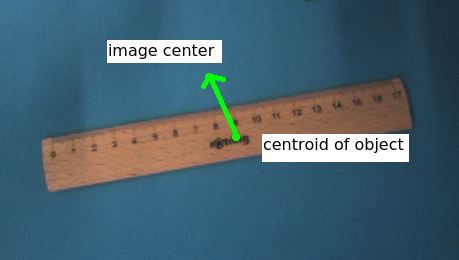
\includegraphics[width=0.6\linewidth]{vector}
	\caption{\label{fig:state1}Vector points from centroid of object to center of image}
\end{figure}
For tabular Q-learning, state space is designed as length and angle of this vector.  We discrete the length into 100 intervals and angle into 36 bins. The learning is run in the MLR code base for 20000 iterations. Test shows that the policy works in simulation while the dynamic of state transition on real robot is different with simulation and the policy fail most of the time. 
\begin{figure}[!htb]
	\centering
	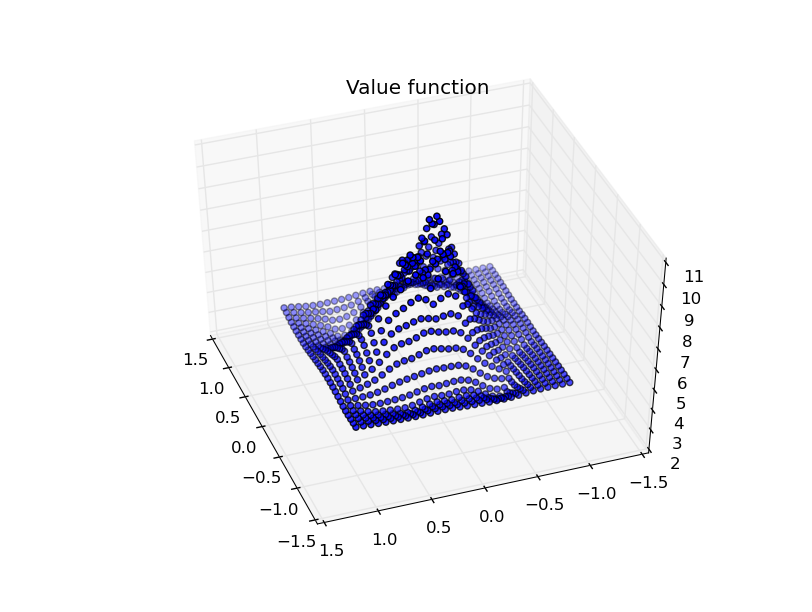
\includegraphics[width=0.9\linewidth]{value}
	\caption{\label{fig:value}Value function of LSPI}
\end{figure}
\begin{figure}[!htb]
	\centering
	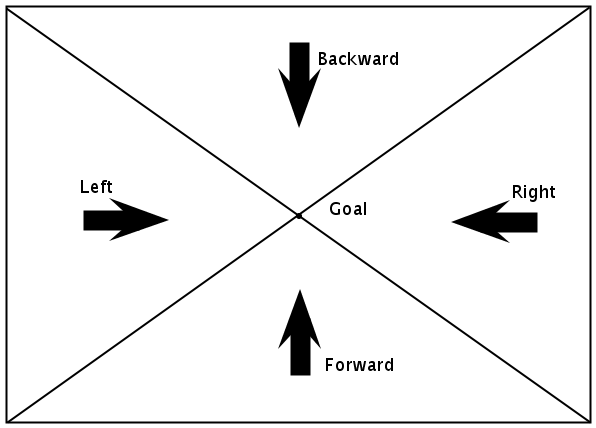
\includegraphics[width=0.7\linewidth]{policy.png}
	\caption{\label{fig:policy}Illustration of policy from LSPI}
\end{figure}

Next we try LSPI. We divide the image into 201x201 grids and the vector is mapped to a grid index (x,y). The learning is run in python. Figure \ref{fig:value} and \ref{fig:policy} shows the value function and a illustration of policy. The policy try to reduce the vector to $\vec{0}$.

The policy from LSPI works well on Baxter, but it is slow in moving because of step size. So we include Aruco marker\cite{c11}. Baxter first tries to detect marker on camera image and estimate the position of the marker. If the marker is not detected, the policy will be used to track the center of object until a marker is detected. Figure \ref{fig:marker} shows a object with Aruco marker.

Finally, the arm moves to a position where is about 20cm above the marker. 
\begin{figure}[!htb]
     \centering
     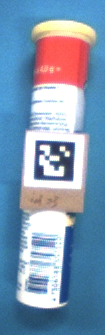
\includegraphics[width=0.1\linewidth]{marker}
      	\caption{\label{fig:marker}Object with Aruco marker}
      \end{figure}
\subsection{Choose grasping point}
Once the robot arm moved to the position above, we continue with the detection of grasping point. We follow the method of Jeannette Bohg and Danica Kragic\cite{c4} in order to learn grasping points with shape context\cite{c5}. We also use synthetic labelled images from the database generated by Stanford University\cite{c6}. We examine two supervised learning algorithms, a linear classifier (logistic regression) and a non-linear classifier (Support Vector Machines (SVMs))\cite{c9}. Data extracting and training parts are implemented in Python.

\subsubsection{Feature vector}
By applying the Canny edge detector, we get the edge of the object. After that, we subdivide the image into rectangular patches of 10x10 pixels. A descriptor for each patch is used to decide whether it represents a grasping point or not. We sample the edges of each patch into 300 points. Four angle and five log radius bins are employed for the shape context histogram. The three histograms in three different scales centered at the current patch are concatenated to form the final feature descriptor of dimension 60.

\subsubsection{Training database}
We train the classifier by the set of \textit{Pencils, white board erasers and martini glasses}. 

In our case, the data set has a strong class imbalance. To be detailed, the number of non-grasping point samples is much larger than grasping point samples. This imbalanced data  can mislead some classification algorithms. In order to tackle this problem, we balance the data set by choosing the same amount of samples from the majority class and the minority class. The main goal is to convert the imbalanced classification data set into a balanced classification data set so the regular classification algorithms can be used.
\subsubsection{Classification methods}
We use \textit{scikit-learn}\cite{c7} for training the Logistic regression linear model and applying SVMs.
\paragraph{Logistic regression}
We denote the binary variable for an image patch in the image by the value of 1 or -1 for being a grasping point or not. After that, we determine coefficient of the features by using \textit{scikit-learn}
\paragraph{Support Vector Machines}
In order to apply SVMs, we need to solve the following optimization problem:
$$max\sum_{i}\lambda_i-\frac{1}{2}\sum_{i,j}\lambda_i\lambda_j g_i g_jK(D_i,D_j)$$
$$s.t \ 0 \leq \lambda_i \leq C$$
$$\sum_i\lambda_ig_i=0$$
Where$D$ is feature descriptor and $g$ is the label. $\lambda$ is the Lagrange multiplier.

We choose non-linear \textit{Radial Basis Function} as a kernel of SVMs:
$$K(D_i,D_j)=e^{-\gamma\|D_i-D_j\|^2}$$ 

There are two parameters for an RBF kernel: $C$ and $\gamma$. It is not known beforehand which pair of $C$ and $\gamma$ are best for a given problem. To identify good parameters for SVMs, we use grid search\cite{c8} over a 5 x 5 parameter space.

\paragraph{Test result}We test the classifier on both synthetic objects and real objects. The result is shown in table \ref{tab:syntheticobject} and \ref{tab:realobject}.
\begin{table}[!htb]
	\centering
	\caption{Accuracy of the Logistic Regression model, testing on synthetic objects}
	\label{tab:syntheticobject}
	\begin{tabular}{c|c|c}
		\hline
		\textbf{Martini Glass} & \textbf{Eraser} & \textbf{Thick Pencil} \\ \hline
		77.34\%                & 58.08\%         & 79.58\%               \\ \hline
	\end{tabular}
\end{table}
\begin{table}[!htb]
	\centering
	\caption{Accuracy of the Logistic Regression model, testing on real objects}
	\label{tab:realobject}
	\begin{tabular}{c|c}
		\hline
		\textbf{Screwdriver} & \textbf{Cylinder-shape Objects} \\ \hline
		76.84\%              & 77.42\%                         \\ \hline
	\end{tabular}
\end{table}






\subsection{Estimate position and orientation}
After getting the grasping point from B, we first try stereo matching to estimate the 3D position of grasping point. The left arm camera takes two pictures at different positions and reconstructs the depth map from stereo matching. Due to the performance of hand camera and the loose joint of arm, the disparity map is sparse and much information is lost. The position estimation is unstable.

Next, we try the projection relation to estimate the 3D position. Since we use a marker in approaching object, the distance between camera and  marker is known. As shown in figure \ref{fig:pos}, we can estimate the $X$ coordinate of grasping point in world frame by the following equation(estimate $Y$ is similar). Vertical distance from camera center and marker, $Z$ is 20cm, focal length $f$ is known and the distance in x axis between grasping point and image center, $x$ is also known. 
$$\frac{x}{X}=\frac{f}{Z}$$
\begin{figure}[!htb]
	\centering
	\includegraphics[width=.6\linewidth]{pos}
	\caption{\label{fig:pos}3D position estimation}
\end{figure}

Additionally, a patch around grasping point will be cut from image. This patch is used in SIFT\cite{c10} feature tracking to track the grasping point in image. The reason is that after 3D position is estimated, due to error in estimation, the grasping may fail and displace the object. Thus old 3D position is useless. SIFT feature tracking updates the center of patch and 3D position of grasping point is re-estimated.

To estimate the orientation, we fit a rectangle to the contour of object. Possible grasping orientation is defined as the two axises of this rectangle, shown in figure \ref{fig:ori}. Since it is more possible to grasp from the narrow side of rectangle. The axis which is perpendicular to narrow side is chosen(long axis in figure).
\begin{figure}[!htb]
	\centering
	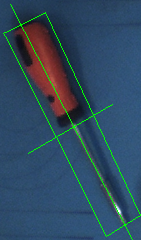
\includegraphics[width=.3\linewidth]{ori}
	\caption{\label{fig:ori}Orientation estimation}
\end{figure}
\subsection{Execute grasping} 
After orientation and position are estimated, the arm will move to the estimated gasping point and try closing gripper. Then the force sensor in gripper is checked, if the force is larger than a defined threshold(10\% max force), then Baxter will lift the object and check force sensor again. If sensor reading is still larger than threshold, it is a successful grasping.

While the estimation error of position and orientation may cause grasping failure, then the arm will repeat A,B,C,D. If it fails more than five times, the arm will grasp the object by visual servoing using the policy from A. The overall logic is shown in figure \ref{fig:logic}
\begin{figure}[!htb]
	\centering
	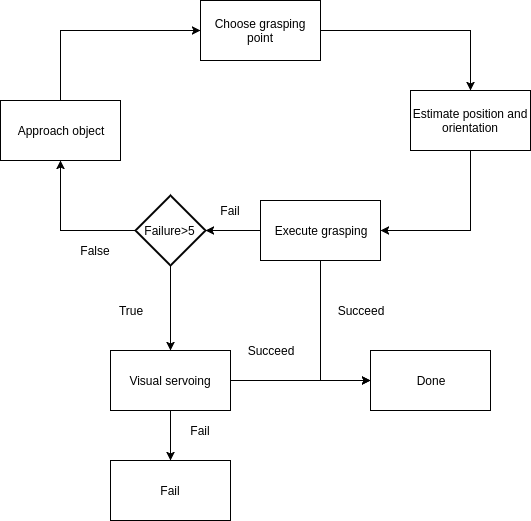
\includegraphics[width=.8\linewidth]{logic}
	\caption{\label{fig:logic}Grasping logic}
\end{figure}

We test Baxter to grasp real object(whole grasping task), stampler, cylinder and screwdriver. Table \ref{grasptime} shows the number of attempts Baxter grasp a single object successfully. One means Baxter grasp object at the first attempt.  
\begin{table}[!htb]
	\centering
	\caption{Number of attempts before Baxter grasp successfully different objects}
	\label{grasptime}
	\begin{tabular}{c|c|c|c}
		
		\textbf{Test No.} & \textbf{Screwdriver} & \textbf{Cylinder-shape Object} & \textbf{Stampler} \\ \hline
		1)                & 1                    & 1                 & 1                \\ 
		2)                & 1                    & 1                 & 3                \\ 
		3)                & 1                    & 1                 & 1                \\ 
		4)                & 1                    & 1                 & 1                \\ 
		5)                & 1                    & 1                 & 2                \\ 
		6)                & 1                    & 1                 & 1                \\ 
		7)                & 1                    & 1                 & 1                \\ 
		8)                & 2                    & 3                 & 1                \\ 
		9)                & 1                    & 1                 & 1                \\ 
		10)               & 2                    & Failed               & 2                \\ 
	\end{tabular}
\end{table}
 
\section{DISCUSSION}
In our proposal, we described the system as using reinforcement learning to make Baxter robot learn to grasp actual object in an efficient way. Using reinforcement learning in performing the whole grasping task(without dividing into subtasks) is far beyond our knowledge. Instead of that, we train the movement of robot's arm in 2D plane, then apply computer vision techniques to estimate the depth map of object in world coordinate. The policy works well, however, it quickly turns out that the policy is quite simple, which is illustrated in Fig. \ref{fig:policy}. Therefore, we upgrade the complexity of out project by adding the work of choosing grasping point using machine learning approach. 
\section{CONCLUSIONS}
By applying several techniques of reinforcement learning, computer vision and machine learning, we are able to make Baxter robot grasp a single object successfully. Our experimental result demonstrate that our method can grasp objects similar to training samples and some objects not seen during training.
 
In the near future, our project can be extended to multiple objects grasping with object clutter in one workspace and using deep learning such as convolution neuron networks for detecting grasping point.


\addtolength{\textheight}{-12cm}   % This command serves to balance the column lengths
                                  % on the last page of the document manually. It shortens
                                  % the textheight of the last page by a suitable amount.
                                  % This command does not take effect until the next page
                                  % so it should come on the page before the last. Make
                                  % sure that you do not shorten the textheight too much.

%%%%%%%%%%%%%%%%%%%%%%%%%%%%%%%%%%%%%%%%%%%%%%%%%%%%%%%%%%%%%%%%%%%%%%%%%%%%%%%%



%%%%%%%%%%%%%%%%%%%%%%%%%%%%%%%%%%%%%%%%%%%%%%%%%%%%%%%%%%%%%%%%%%%%%%%%%%%%%%%%



%%%%%%%%%%%%%%%%%%%%%%%%%%%%%%%%%%%%%%%%%%%%%%%%%%%%%%%%%%%%%%%%%%%%%%%%%%%%%%%%

%%%%%%%%%%%%%%%%%%%%%%%%%%%%%%%%%%%%%%%%%%%%%%%%%%%%%%%%%%%%%%%%%%%%%%%%%%%%%%%%





\begin{thebibliography}{99}

\bibitem{c1}Pinto, Lerrel, and Abhinav Gupta. "Supersizing self-supervision: Learning to grasp from 50k tries and 700 robot hours." Robotics and Automation (ICRA), 2016 IEEE International Conference on. IEEE, 2016.
\bibitem{c2}Watkins, Christopher JCH, and Peter Dayan. "Q-learning." Machine learning 8.3 (1992): 279-292.
\bibitem{c3}Lagoudakis, Michail G., and Ronald Parr. "Least-squares policy iteration." Journal of machine learning research 4.Dec (2003): 1107-1149.
\bibitem{c4}Jeannette Bohg and Danica Kragic. "Learning grasping points with shape context." Robotics and Autonomous Systems, Volume 58, Issue 4, 30 April 2010, Pages 362-377.
\bibitem{c5}S. Belongie, J. Malik, J. Puzicha. "Shape matching and object recognition using shape contexts." IEEE Transactions on Pattern Analysis and Machine Intelligence 24(4) (2002) 509-522.
\bibitem{c6}A. Saxena, J. Driemeyer, J. Kearns, A.Y. Ng. "Robotic grasping of novel objects." Neural Information Processing Systems 19 (2007) 1209-1216.
\bibitem{c7}Pedregosa et al. "Scikit-learn: Machine Learning in Python." JMLR 12, pp. 2825-2830, 2011.
\bibitem{c8}Chih-wei Hsu and Chih-chung Chang and Chih-jen Lin. "A practical guide to support vector classification" 2010.
\bibitem{c9}Cortes, C. and Vapnik, V. (1995). "Support-vector networks". Machine Learning. 20 (3): 273-297
\bibitem{c10}Lowe, David G. "Object recognition from local scale-invariant features." Computer vision, 1999. The proceedings of the seventh IEEE international conference on. Vol. 2. Ieee, 1999.
\bibitem{c11}Garrido-Jurado, Sergio, et al. "Automatic generation and detection of highly reliable fiducial markers under occlusion." Pattern Recognition 47.6 (2014): 2280-2292.





\end{thebibliography}




\end{document}
